% IEEEtran V1.8b, standard conference layout; no geometry or font-size overrides.
\documentclass[conference,letterpaper]{IEEEtran}
\usepackage[T1]{fontenc}
\usepackage{microtype,amsmath,amssymb,booktabs,tabularx,graphicx,xcolor}
\usepackage[hyphens]{url}
\usepackage[hidelinks]{hyperref}
\title{Determinants of Speculative Decoding Efficiency in Resident MoE Inference}
\author{\IEEEauthorblockN{Working research manuscript}
\IEEEauthorblockA{Author names and affiliations pending}}
\begin{document}
\maketitle
\begin{abstract}
Speculative decoding trades fewer target iterations for more work per iteration. Prior work establishes how expert activation and batch size affect this tradeoff in mixture-of-experts (MoE) inference. We characterize additional determinants in a resident single-GPU engine: draft availability, actual verification shape, routing dependence, and the service measurement boundary. Separate eager and compiled BF16 OLMoE/n-gram campaigns each cover seven batch sizes and eight draft caps with two repetitions per cell. An ordinary-decoding routing model predicts distinct experts in held-out speculative executions with mean absolute error 1.91 using actual verification rows, versus 15.30 using the nominal batch--cap product. Matched single-layer replays support distinct-expert cost fits with held-out mean absolute percentage error of 2.35\% eager and 1.92\% with CUDA graphs, without establishing a compute transition. Instrumented compiled execution shows padding enlarging physical expert participation. Eager execution gives small-batch throughput gains; in the separately warmed compiled campaign all 49 speculative cells fall below matched ordinary-decoding throughput. Effective token latency can still improve. Different warmup and run windows preclude attributing this contrast solely to graphs. A separate five-policy evaluation finds no aggregate TPOT advantage for full-budget adaptive truncation over selected static ordinary decoding; its large-batch TPOT improvement trades against throughput and energy. A small natural-stop task check does not establish quality equivalence; broader draft/workload validation remains pending.
\end{abstract}
\begin{IEEEkeywords}
Mixture-of-experts, speculative decoding, performance modeling, GPU inference.
\end{IEEEkeywords}

\section{Introduction and Scope}
Speculative decoding trades fewer target iterations for more work per iteration. In resident mixture-of-experts (MoE) inference, extra verification positions can touch experts that ordinary decoding would not use. MoESD already models the resulting batch-dependent opportunity and demonstrates it experimentally~\cite{moesd}. Our narrower question is: \emph{which observed determinants connect a configured draft cap to expert participation, useful progress, and measured service cost?} A qualitative batch reversal alone is not our proposed novelty.

We characterize actual verification shape, draft availability, graph padding, and service measurement boundaries in one resident single-GPU engine. Expert offloading and inter-GPU communication are outside scope. We use n-gram proposals first; compatible neural sources such as EAGLE-3 require separate target, tokenizer, and interface validation~\cite{eagle3,eaglerepo}. The target verifier and sampler retain responsibility for acceptance and token emission; $\gamma=0$ denotes ordinary decoding.

The eager and compiled campaigns each cover 56 batch--cap cells and 112 performance records, with separate routing diagnostics and component replay. Two service repetitions per cell do not establish significance. Route-probability fit and test use different caps but shared prompts. Compiled service measurements exclude detailed route capture. A separate 40-run five-policy evaluation tests the implemented controller against frozen native schedules. It does not support an aggregate advantage in this n-gram domain; a small natural-stop check retains task-quality limitations, and neural sources remain pending.

A selected-expert union measures participation, not HBM traffic: caches, tiles, representation, and dispatch affect physical reads. Likewise, finite synchronous waves that drain without refilling measure burst throughput rather than steady-state serving capacity. We retain these distinctions when relating occupancy, layer time, request latency, and energy.

\section{Model and Predictions}
\subsection{Expert occupancy with top-\texorpdfstring{$k$}{k} routing}
For layer $\ell$, let $R_{\ell,s}$ be the distinct expert IDs selected for valid token slot $s$, $E_\ell$ the routed expert count, and $k_\ell=|R_{\ell,s}|$ when top-$k$ is fixed. Define the per-token inclusion probability
\begin{equation}
q_{\ell,e}=\Pr(e\in R_{\ell,s}),\qquad
\sum_{e=1}^{E_\ell}q_{\ell,e}=k_\ell.
\end{equation}
Linearity of expectation yields the exact identity
\begin{equation}
\mathbb E[D_\ell(S)] = \sum_e\left[1-\Pr\!\left(\bigcap_{s=1}^{S}\{e\notin R_{\ell,s}\}\right)\right].
\end{equation}
If token slots are independent and have stationary inclusion probabilities, this becomes
\begin{equation}\label{eq:d}
\widehat D_\ell(S)=\sum_e[1-(1-q_{\ell,e})^S].
\end{equation}
No independence among the experts selected by one token is required. If a trace instead reports the fraction $p_{\ell,e}$ of all assignments, with $\sum_e p_{\ell,e}=1$, then $q_{\ell,e}=k_\ell p_{\ell,e}$. Treating top-$k$ as $Sk$ independent draws with replacement gives a different model and can violate the exact $D_\ell(1)=k_\ell$ check.

Let $m_{t,i}$ be available draft length and $k_{t,i}\leq\min(m_{t,i},\gamma_t)$ the scheduled prefix for request $i$. An unchunked decode-only call has $S_t=\sum_{i=1}^{B_t}(1+k_{t,i})$ valid rows, including subsequently rejected positions. Nominal $B(\gamma+1)$ is attained only with full prefixes. Chunking, mixed prefill/decode, output limits, and padding are recorded separately. Direct route unions measure $D_\ell$; uniform routing is only a reference, not the measured predictor.

Graph execution can process $P_t\geq S_t$ model-forward rows, excluding expert GEMM tile padding. We record valid, padding-only, and total expert histograms. Extra physical participation need not yield useful progress (Section~\ref{sec:compiled}); neither union directly measures bytes or padding time.

\subsection{From occupancy to complete iteration cost}
Let $w_{\ell,e}$ be expert weight storage bytes in the deployed representation. The logical routed working-set estimate is
\begin{equation}
\widehat W_\ell(S)=\sum_e w_{\ell,e}[1-(1-q_{\ell,e})^S].
\end{equation}
Shared experts are recorded separately. For a fixed layer, precision, and expert kernel, the proposed component fit is
\begin{equation}\label{eq:time}
\widehat T_{\rm MoE}(D,S)=\max(aD,bS)+c,\qquad a,b,c\geq0.
\end{equation}
Here $D,S$ are actual fixed-input replay counts, fitted separately for eager and CUDA-graph execution. Full-model graph padding additionally requires physical rows and unions. The coefficients are local empirical costs, not bandwidth, FLOP rates, or identified overhead components. Imbalance, alignment, cache state, and launch behavior may require richer terms. The $aD+c$ form suffices in both measured execution modes (Section~\ref{sec:kernel}), establishing neither zero compute cost nor full-model fixed-cost dominance.

Component replay tests measured $D,S$ against layer time; Equation~\ref{eq:d} separately tests routes against $D$. Neither validates complete-step time. Attention depends on context, query count, and backend; shared logical KV does not imply constant physical reads. Complete cost therefore uses a separate table indexed by batch, scheduled cap, production budget, and execution regime. The host-step boundary includes target verification, next-draft production, sampling, scheduling, and control, without subtracting guessed components or adding overlapping phases.

\subsection{Accepted work and the decision rule}
Let $M$ be the available draft length before truncation under production budget $G$. For a chosen cap $\gamma\leq G$, distinguish availability $v_j=\Pr(M\geq j)$ from conditional prefix survival $s_j=\Pr(\text{first }j\text{ accepted}\mid M\geq j)$, for $j\leq\gamma$. These probabilities refer to the same state and budget; their product requires no independence assumption. With one correction/bonus token and no terminal or output-budget censoring, expected emitted tokens per request per round are
\begin{equation}\label{eq:a}
A(\gamma;G)=1+\sum_{j=1}^{\gamma}v_j s_j.
\end{equation}
Empty proposals contribute no availability but retain lookup/target costs. Availability precedes truncation; ranks beyond $G$ are unobserved. Prefix survival is estimated among requests scheduled to rank $j$, counting earlier rejection as failure. EOS/output-cap-censored cases are excluded from this uncensored estimator but retained in population reports.

Full availability and rank-invariant conditional acceptance $\alpha_g$ yield $1+\alpha_g+\cdots+\alpha_g^\gamma$. The code's scalar $\bar\alpha=C_a/C_n$ instead pools reached positions: $a=\sum_i a_i$ and $n=\sum_i\min(a_i+1,k_i)$ for accepted-prefix lengths $a_i$ and scheduled lengths $k_i$. Positions after first rejection are untested. Counts update as $C_a\leftarrow0.9C_a+0.1a$, $C_n\leftarrow0.9C_n+0.1n$, with prior $(0.7,1)$; zero-exposure steps neither update nor decay. This pooled ratio need not equal a rank's conditional probability. The policy primarily uses empirical prefix survival and availability; $\bar\alpha$ supplies initial/unseen-rank geometric priors. Prefix/availability EWMAs weight eligible-step proportions; count decay is also per eligible step, not elapsed time. Unseen availability starts at one; priors, rank-population changes, and monotone projection require validation.

For a stable batch and matched ordinary-decoding baseline,
\begin{equation}\label{eq:speed}
\widehat{\rm Speedup}(B,\gamma)=
\frac{\widehat A(\gamma;G)\widehat T_{\rm round}(B,0;0)}
{\widehat T_{\rm round}(B,\gamma;G)}.
\end{equation}
The online action is selected from a small supported set $\Gamma$ including zero:
\begin{equation}\label{eq:policy}
\gamma_t^*=\arg\max_{\gamma\in\Gamma}
\frac{\widehat A_t(\gamma;G)}
{\widehat T_{\rm round}(B_t,\gamma;G,L_t)}.
\end{equation}
The causal policy uses recent availability/survival and offline complete costs, with ties favoring shorter caps. Context can be fixed or binned. Native production uses the selected budget; post-proposal integration holds $G$ fixed and pays its full cost even at $\gamma=0$. Section~\ref{sec:controller} evaluates this rule as an executed policy, including its production and graph configuration.

\paragraph{Testable scope} Larger AR working sets can reduce relative verification expansion, but compute, attention, and drafting still grow or persist. Occupancy and component timing are separate tests; complete-cost action ranking and service improvement require actual held-out policy execution.

\section{Measured Characterization}\label{sec:characterization}
\subsection{Setting and population}
Both campaigns use OLMoE-1B-7B-0924-Instruct (revision \texttt{7f1c97f4}), resident BF16 weights, vLLM 0.26.0, and an NVIDIA RTX PRO 6000 Blackwell Server Edition. The MoE backend is Triton, attention is automatically selected, and KV allocation is 6\,GiB. Each covers $B\in\{1,2,4,8,16,32,64\}$ and $\gamma\in\{0,\ldots,7\}$: 56 cells, two runs each. All 224 runs complete the same 64 ShareGPT-derived requests with 128 forced tokens (8,192 total/run). Service runs exclude detailed route capture.

Eager r02 warmed only $B=64$; compiled r01 enables V1 graphs, scheduler cap 64, and 32-token warmup for each batch/prompt shape. GPU lock occupancy is 3,091.24/2,223.79\,s, including startup/warmup (and eager diagnostics). Different warmup and execution windows prevent a graph-only causal comparison. Ratios use two-run medians, retaining raw values and order effects. Waves drain without refilling; throughput divides tokens by summed wave windows (submission, prefill, decode, and drain), excluding inter-wave gaps. These are finite-burst observations, not steady-state capacity or significance estimates.

\begin{figure*}[t]
\centering
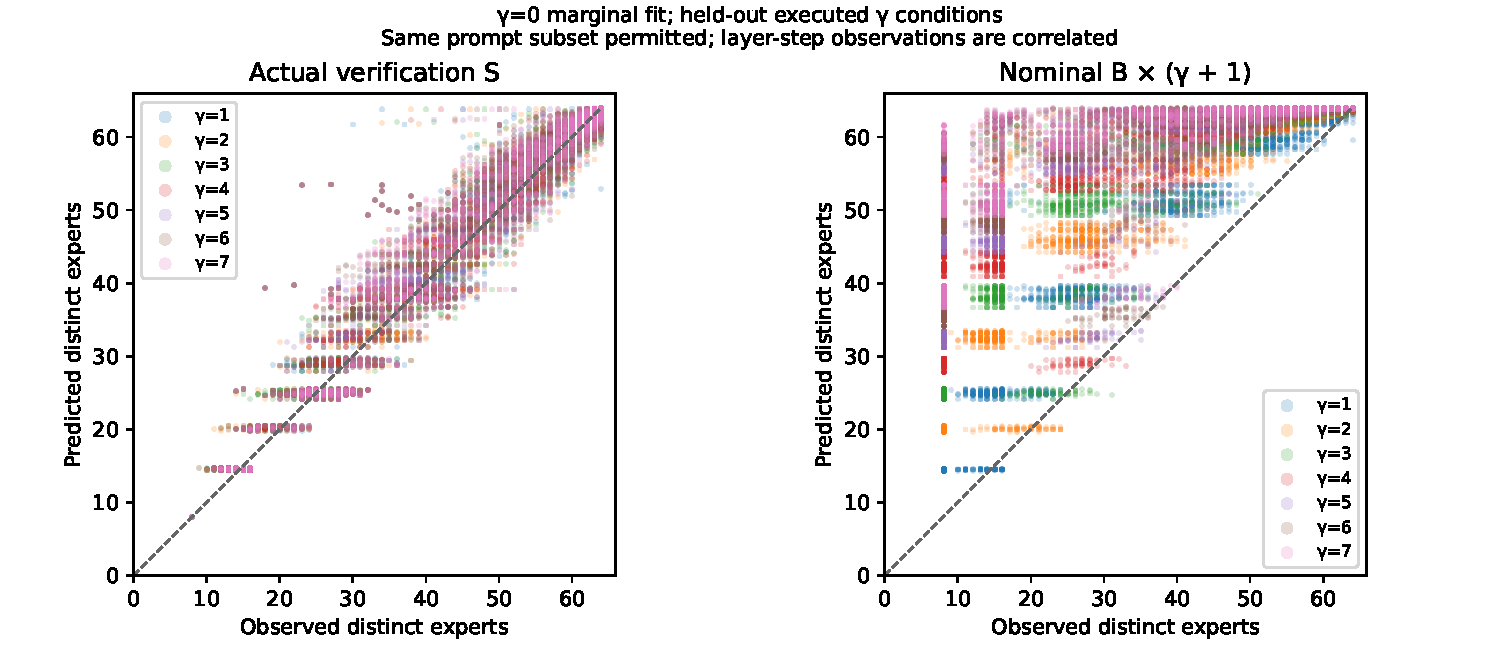
\includegraphics[width=\textwidth]{../figures/F1_olmoe_ngram_r02/route_prediction_scatter.pdf}
\caption{F1: expert-occupancy prediction using the same AR-fitted inclusion probabilities $q_e$ in both panels. Left uses actual valid verification rows $S$; right uses nominal $B(\gamma+1)$. Fit: 3,472 AR layer-step observations. Test: 23,568 observations from $\gamma=1$--$7$ executions, including rejected draft positions. The prompt subset is shared, so this is held-out execution-condition validation, not independent-workload validation. All eligible decode points, including the first step, remain in both panels. Logical expert counts do not measure HBM traffic or time.}
\label{fig:f1}
\end{figure*}

\subsection{Actual shape predicts participation better than the configured cap}
We fit layerwise, token-weighted inclusion probabilities from $\gamma=0$ across all seven batches and test $\gamma=1$--$7$. Decode-only histograms satisfy top-$k$ conservation and include rejected positions; prefill/mixed steps are excluded. The 3,472 fit and 23,568 test layer-steps share prompts and are correlated, not independent system samples.

Actual $S$ gives MAE 1.9145 experts and RMSE 3.1453 (Figure~\ref{fig:f1}); nominal $B(\gamma+1)$ raises MAE to 15.2994 with the same $q_e$. Actual active batch with nominal cap still gives 13.6975, so correcting wave tails alone is insufficient. This isolates shape input, not nonuniform versus uniform routing, and validates neither independent-workload transfer nor action ranking.

\paragraph{Structured residuals} First decode steps contribute 784/23,568 observations (3.33\%) but 25.78\% of squared error: MAE is 5.73 versus 1.78 later. All remain included. AR layer 0 at $B=32$ also starts at 26 distinct experts versus 61.07 afterward. First decode processes the first generated token, not directly a template token; shared templates or repeated identities are untested explanations, not draft-specific causes.

\begin{figure*}[t]
\centering
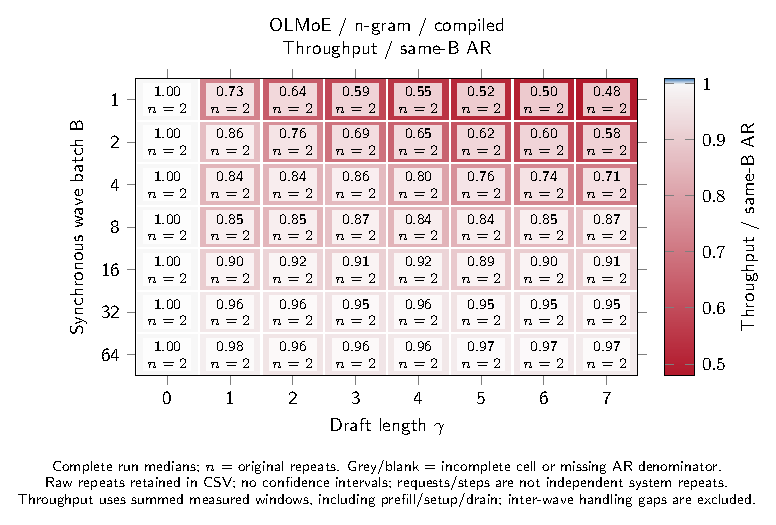
\includegraphics[width=0.82\textwidth]{../figures/F2_olmoe_ngram_compiled_r01/speedup_15c7a01f28d9.pdf}
\caption{F2: complete compiled r01 finite-wave throughput, normalized to compiled AR at the same initial batch. Each of 56 cells has two repetitions after per-shape warmup; all 49 speculative ratios are below one. Windows include prefill and wave drain. Ratios are descriptive, not significance estimates. Eager r02 is retained as a separate historical campaign.}
\label{fig:f2}
\end{figure*}

\subsection{Throughput and request token latency answer different questions}
Compiled r01 gives throughput ratios 0.479--0.727$\times$ at $B=1$, 0.580--0.864 at $B=2$, 0.711--0.857 at $B=4$, and 0.841--0.874 at $B=8$ (Figure~\ref{fig:f2}). At $B=16,32,64$, ranges are 0.892--0.918, 0.950--0.962, and 0.958--0.979. All 49 speculative cells are below AR; this low-availability n-gram setting does not become faster at medium batch. This is an observed campaign direction, not a universal reversal or significance claim.

Eager r02 remains distinct: $B=1,2,4$ give 1.129--1.179, 1.061--1.107, and 1.025--1.066$\times$; all $B=16,32$ cells are at or below AR, and $B=64$ spans 0.995--1.028. Its cold-shape effects and separate run window preclude assigning this contrast solely to graphs or padding. Neither campaign satisfies the full-availability, constant-$\alpha_g=0.7$ illustration, which supplies no calibrated crossover.

Effective TPOT averages each request's first-to-last emitted-chunk interval divided by 127, then takes the run median. It can improve more than wave throughput (Table~\ref{tab:objectives}); early finishers leave unfilled slots while the wave waits for its last request.

An eager-r02 receipt decomposition separates mean first receipt, mean post-first span, and the barrier $\max_i(\mathrm{last}_i)-\mathrm{mean}_i(\mathrm{last}_i)$. Summed over 64-request waves and averaged over runs, $\gamma=6$ versus AR at $B=16$ changes these terms by $-0.00436$, $-0.70788$, and $+0.71303$\,s; at $B=64$ by $+0.000305$, $-0.25573$, and $+0.20864$\,s. Initial receipt growth does not explain this eager gap. The barrier is not a recoverable-time bound: refill changes execution. Matched queued service and kernel/fixed-cost attribution remain pending.

\begin{table}[t]
\centering\small
\caption{Different objectives within each execution campaign. Ratios compare two-run medians with matched AR. TPOT speedup is AR time divided by speculative time; throughput speedup is speculative rate divided by AR rate.}
\label{tab:objectives}
\begin{tabular}{@{}lrrrr@{}}
\toprule
Mode & $B$ & $\gamma$ & Throughput & TPOT \\\midrule
Eager & 16 & 6 & 0.9999$\times$ & 1.1299$\times$ \\
Eager & 64 & 6 & 1.0234$\times$ & 1.1582$\times$ \\
Compiled & 64 & 6 & 0.9656$\times$ & 1.0702$\times$ \\
\bottomrule
\end{tabular}
\end{table}

Compiled TPOT speedup exceeds one in 15 cells ($B=16,\gamma=4$ and all positive caps at $B=32,64$), while all throughput ratios remain below one. Including inter-wave gaps in the full-population denominator preserves that throughput direction. Raw pairs remain important: eager $B=1$ AR is $(82.55,87.75)$ versus $(95.69,96.63)$ tokens/s for $\gamma=1$; compiled $B=64$ AR is $(4746.20,4796.94)$ versus $(4684.17,4530.96)$ for $\gamma=6$. Near-unity cells require their run variation and warmup context.

\subsection{Draft availability and progress}
All eager-r02 performance decode request-steps, including empty proposals, tails, and terminal steps, enter Figure~\ref{fig:f5}. At $B=1$, nonempty-proposal rates for $\gamma=1,4,7$ are 18.07/14.09/13.37\%; mean draft slots are 0.181/0.562/0.928, and emitted tokens are 1.095/1.149/1.158. These are unconditional population rates, not acceptance conditioned on an n-gram hit or the pooled scalar $\bar\alpha$.

Cap alone therefore poorly represents verification work; acceptance without availability cannot predict progress. Lookup, target, and wave costs still determine throughput. Terminal/output limits can make $1+$accepted drafts differ from client emission, so both are retained.

Cold-prior-per-run offline replay changes the $B=1,\gamma=7$ scalar estimator's tested-position-weighted pre-step bias from $-0.2285$ to $-0.0137$ when replacing EWMA step ratios with EWMA count ratios. Progress MAE stays near 0.282 tokens because availability/prefix weighting is unchanged. Both versions are retained; this is statistical correction on fixed traces, not adaptive execution or performance gain.

\begin{figure*}[!t]
\centering
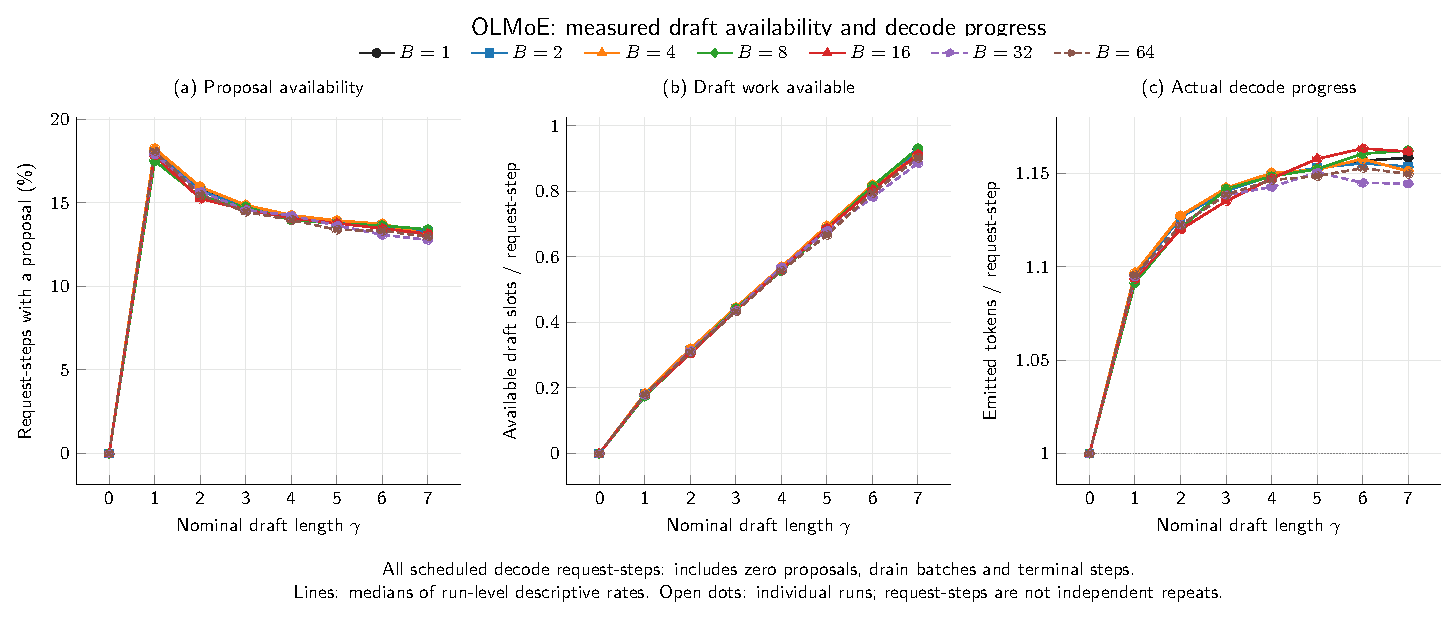
\includegraphics[width=\textwidth]{../figures/F4F5_olmoe_ngram_r02/F5_availability_progress.pdf}
\caption{F5 eager-r02 coverage/progress component: nonempty proposal frequency, mean available draft slots, and actual client-emitted tokens per decode request-step. All 112 performance records contribute, including empty drafts, shrinking drain batches, and terminal steps. Lines summarize two run-level rates and open markers retain their raw values; request-steps are not independent repetitions. This is not a conditional-survival distribution or EWMA-validation plot.}
\label{fig:f5}
\end{figure*}

\begin{figure*}[!t]
\centering
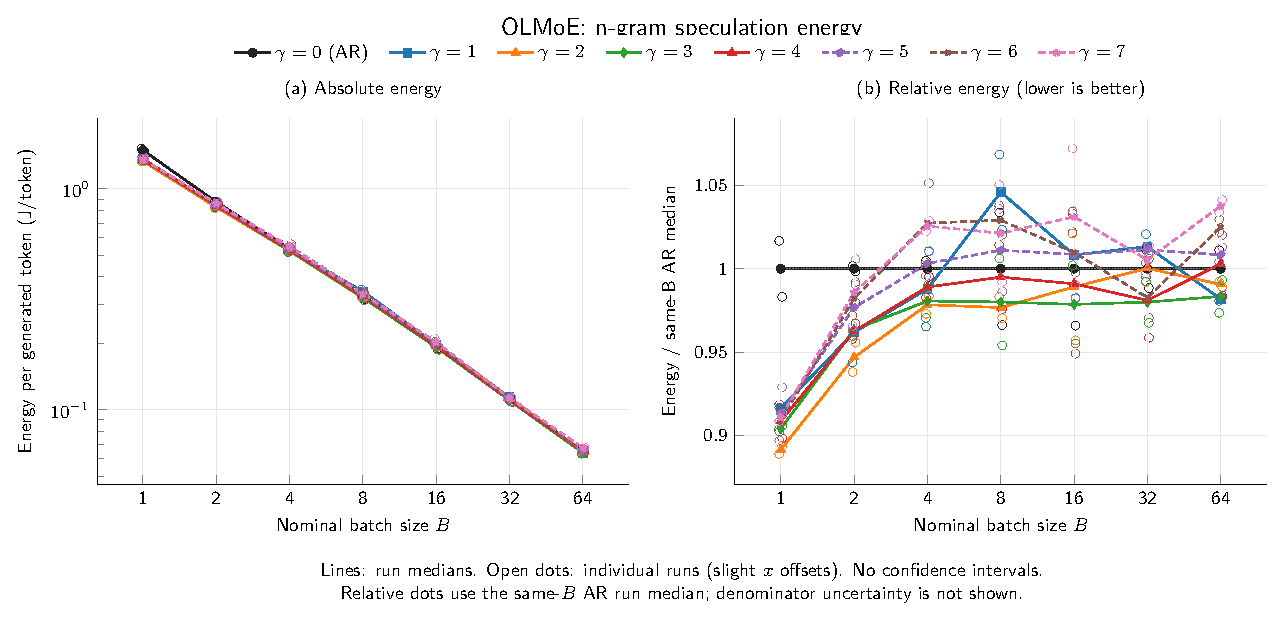
\includegraphics[width=\textwidth]{../figures/F4F5_olmoe_ngram_r02/F4_energy_vs_batch.pdf}
\caption{F4 eager r02: GPU joules per emitted token over the complete wave windows, including prefill. Lines are two-run medians; open markers are raw runs. Right-panel points divide each run by the same-batch AR median, without paired-run inference, confidence intervals, or denominator uncertainty. NVML device energy is neither whole-system nor idle-subtracted energy; different caps need not optimize throughput and energy simultaneously.}
\label{fig:f4}
\end{figure*}

\subsection{Energy is a separate measured objective}
Eager-r02 energy comes from the cumulative NVML device counter over each measured wave, with no idle-baseline subtraction. At $B=1$, AR uses 1.4982\,J/token; speculative caps use 1.3357--1.3728\,J/token (Figure~\ref{fig:f4}). At $B=64$, AR uses 0.0650\,J/token and speculative caps span 0.0638--0.0675\,J/token. For example, $\gamma=6$ at $B=64$ has throughput ratio 1.0234 but uses 0.0666\,J/token. Energy and throughput have different observed orderings. Compiled wave-window J/token exceeds its AR baseline in all 49 speculative cells; including inter-wave gaps in the counter span preserves this direction. Small differences inherit the two-repeat and execution-window limitations.

\begin{figure*}[t]
\centering
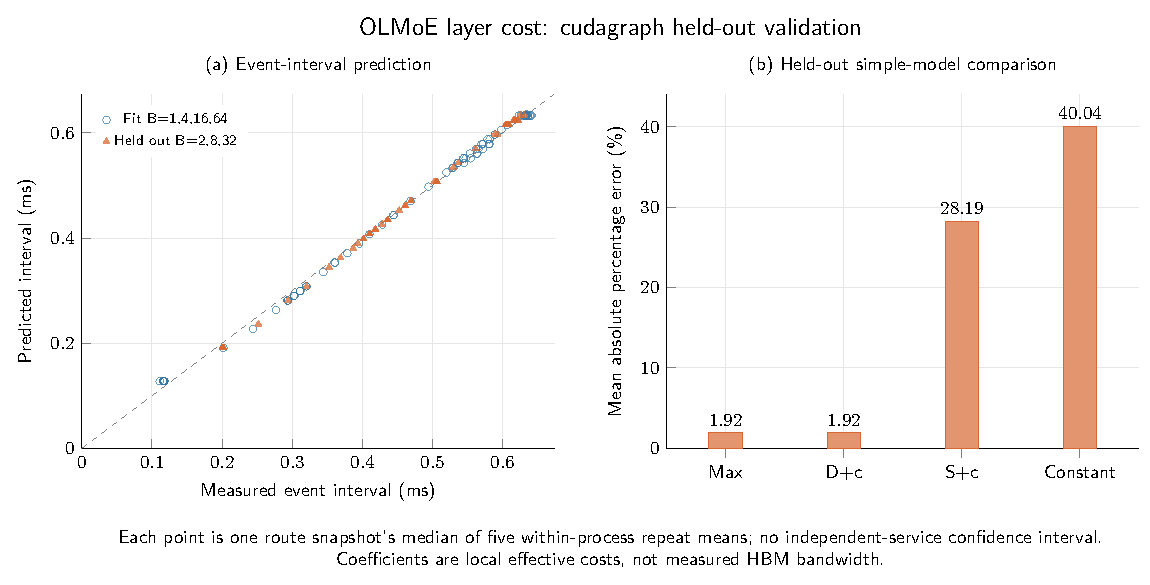
\includegraphics[width=0.90\textwidth]{../figures/kernel_cost_graph_r01/kernel_cost_validation_258f5f5f.pdf}
\caption{Single-layer CUDA-graph cost validation with measured $D,S$: 88 calibration and 66 held-out snapshots use disjoint batches. Points are medians of five within-process repeat means, not independent service runs. The max-form and $aD+c$ have almost equal held-out error; only one calibration point activates the token-count branch.}
\label{fig:kernel}
\end{figure*}

\subsection{Distinct experts predict a measured layer interval}\label{sec:kernel}
The eager r03 and CUDA-graph r01 replays use OLMoE layer 0's resident BF16 weights and vLLM \texttt{TritonExperts}. All 154 cases match in route histograms, synthetic unit-RMS activations/co-occurrence, seeds, uniform top-$k$ weights, kernel, and tile settings; $S=1$--148 and $D=8$--64. Routing quantiles/row extremes select snapshots before timing. Each uses ten warmup calls and five repeats of twenty calls, summarized by the median repeat mean. Both apply 256\,MiB unrelated-buffer turnover outside timers; this does not guarantee identical physical cache contents. All graph captures and recorded warmup-output checks pass.

CUDA events cover preparation, alignment, two expert GEMMs, activation, and reduction, excluding routing, attention, drafting, and scheduling. Each mode independently fits 88 snapshots at $B=1,4,16,64$ and tests 66 at $B=2,8,32$, retaining outliers. Eager $aD+c$ gives $a=9.471$\,$\mu$s/expert, $c=153.261$\,$\mu$s, MAE 12.731\,$\mu$s, and MAPE 2.345\%. Graph $aD+c$ gives $a=9.019$, $c=55.733$ in the same units, MAE 5.868\,$\mu$s, and MAPE 1.924\%. Graph max-form MAPE is 1.920\%, with 87/88 fit points and all test points on the $D$ branch (Figure~\ref{fig:kernel}). Token-count-plus-intercept/constant MAPE is 21.673/29.517\% eager and 28.186/40.041\% graph. The tiny max-form increment does not establish a broad compute regime.

Across matched cases, graph/eager event ratios have median 0.7924 and range 0.4899--0.8669; the wall-time ratio median is 0.7943. All 154 graph intervals are lower. Capture and first replay are excluded and recorded separately. These separately timed campaigns are not randomized/interleaved independent repetitions: the ratios describe an execution-mode contrast, not isolated CPU launch cost or service speedup.

Fixed-layer capture excludes model padding, routing, and attention. Neither fit measures HBM bytes or identifies full-model $c_0$; the eager token branch is unidentified and graph support is limited to one calibration point. Eager profiling omitted turnover; graph profiling includes it; neither profiler differences nor event-minus-profiler gaps isolate CPU overhead. These component fits do not validate complete-step ranking or controller benefit.

\begin{figure*}[t]
\centering
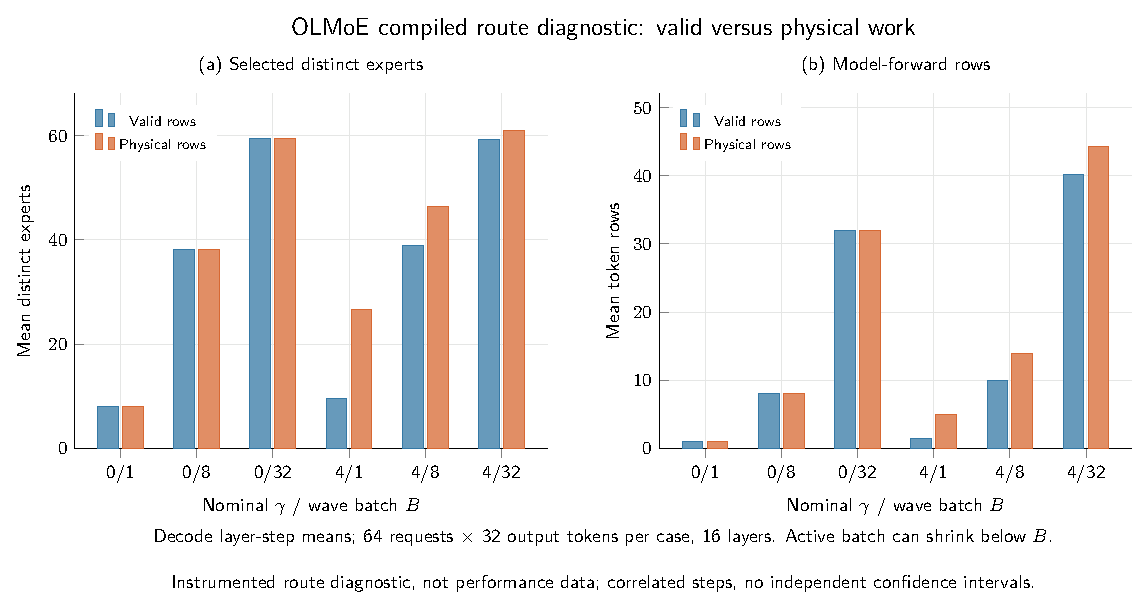
\includegraphics[width=0.84\textwidth]{../figures/compiled_routes_r01/compiled_routes.pdf}
\caption{Instrumented compiled route diagnostic. Physical model-forward rows include graph padding and can activate experts beyond the valid-row union; expert matrix-multiplication tile padding is excluded. Means weight every decode layer-step equally, including shrinking wave tails. The six cases are correlated route observations, without independent confidence intervals or service-time inference.}
\label{fig:compiled}
\end{figure*}

\subsection{Physical participation under graph padding}\label{sec:compiled}
The compiled diagnostic runs $\gamma\in\{0,4\}$ at $B\in\{1,8,32\}$, each with 64 unique requests and 32 forced tokens (Figure~\ref{fig:compiled}). All 16 layers and steps pass top-$k$, histogram, $S$, and $P$ conservation. AR uses FULL dispatch with $S=P$. At $\gamma=4,B=1$, 1,569/1,747 calls use PIECEWISE with $S=1,P=5$; the rest use FULL with $S=P=5$. Mean valid-to-physical $D$ rises 9.62 to 26.73. At $B=8,32$, all calls are PIECEWISE; 224/248 and 54/62 are padded, with mean $D$ rising 38.91 to 46.36 and 59.27 to 60.90.

The \href{https://github.com/vllm-project/vllm/blob/v0.26.0/vllm/config/compilation.py}{native V1 graph-size construction} rounds capture sizes to multiples of engine limit $G_{\rm eng}+1$ only when decode mode is FULL and the uniform query length exceeds one. These fixed-cap diagnostic engines have $G_{\rm eng}=\gamma$; nonuniform calls reuse their rounded table. OLMoE already uses V1, so routed-expert return does not change this dispatch; the observer reads buffers after the call. The same resolved mode/grid and shape imply the same padding rule without tracing, but measured unions and times do not transfer. The diagnostic scheduler cap is 32 versus service cap 64. Native batch tables resolve differently (Section~\ref{sec:native}). Instrumentation establishes participation, not HBM traffic, padding time, or service benefit.

\paragraph{Physical-row prediction} Fitting $q_e$ on compiled AR at $B=1,8,32$ (5,952 tokens/layer) and testing $\gamma=4$ on shared prompts gives valid-$D$ MAE 0.566/3.438/1.946 from $S$. For physical $D$, replacing $S$ with $P$ reduces MAE from 17.675/6.307/1.818 to 3.133/2.898/1.464. These correlated observations hold out execution conditions, not workloads. At $B=1$, residual bias is $+2.562$ and MAPE 12.864\%. All 21,920 adjacent padded layer-step pairs within waves have identical padding histograms. Temporal repetition does not test within-call independence; padding marginals also differ from AR, leaving fresh IID-AR padding unvalidated. Histogram equality proves neither ordered token replay nor cache hits.

% Action-level comparison from the already reviewed primary sources in refs.bib.
% This is not a numerical reproduction or a claim of matched cost accounting.
\begin{table*}[t]
\centering\small
\caption{T2: action-level comparison. Published mechanisms and native capabilities are distinguished from the five implemented comparison arms; this table is not a numerical reproduction of the cited systems.}
\label{tab:t2actions}
\begin{tabularx}{\textwidth}{@{}>{\raggedright\arraybackslash}p{0.14\textwidth}>{\raggedright\arraybackslash}p{0.26\textwidth}>{\raggedright\arraybackslash}p{0.25\textwidth}>{\raggedright\arraybackslash}X@{}}
\toprule
Work & Information & Action / execution scope & Drafting-cost boundary \\\midrule
MoESD~\cite{moesd} & Batch, expert activation, acceptance, fitted cost parameters & Performance model and fixed-$\gamma$ runs; no online optimal-$\gamma(B)$ system located in our reviewed evidence & Fixed-cap drafting and verification; an online selector is not evaluated here. \\
Cascade~\cite{cascade} & Measured iteration utility / useful-token rate & Online test-and-set, disable/restart, back-off, and hill-climbing; original vLLM 0.6.6 implementation & Utility accounts for draft/target iteration work; online probing also incurs cost. Not reproduced here. \\
AdaEAGLE~\cite{adaeagle} & Token embedding and target hidden state; trained predictor & Lightweight MLP predicts next-round draft length & Predictor and actual neural drafting cost; requires predictor training. Not reproduced here. \\
vLLM 0.26~\cite{vllmdynamic,vllmconfig} & Active batch and configured inclusive intervals & Native static cap, threshold, or unrestricted nonmonotone cap table, including zero & Selected cap controls production budget; native execution and scheduling costs remain. \\
This study & Active batch, observed availability/survival, calibrated complete costs & Prefix truncation after a fixed-budget proposal; target routing and verifier retained & Full $G$ cost is paid even at $\gamma=0$; adaptive decision CPU is timed, while total observer perturbation remains unisolated. \\
\bottomrule
\end{tabularx}
\end{table*}

\section{Controller Evaluation and Boundaries}\label{sec:controller}
\subsection{Native controls and complete drafting cost}\label{sec:native}
vLLM 0.26.0 supports inclusive batch intervals mapped to caps, including zero and nonmonotone schedules~\cite{vllmdynamic,vllmconfig}. The five executed arms are AR, selected native static cap, native threshold, unrestricted native batch table, and the batch/EWMA rule. Cascade remains an action-level comparison, not a numerical baseline (Table~\ref{tab:t2actions}). Tables are selected from direct-$\gamma$ development cells, then frozen with $G_{\rm eng}=7$. In V1, configured tables override FULL-containing modes to PIECEWISE and skip the FULL-path $G_{\rm eng}+1$ rounding. Native zero-budget production returns before drafting; adaptive truncation pays for the full proposal. This is a comparison of complete policies and their actual graph/production configurations, not an isolated selection-rule experiment. Selection is neither exhaustive common-graph tuning nor a global optimum; capture logs do not establish timed dispatch or padding costs.

The adaptive controller truncates before scheduler reservation, saving verification rather than already executed drafting. Its compiled $G=7$ cost table has 32 measured cells ($B=1,4,16,64$, caps 0--7), one run each, covering complete synchronous host steps. Small nonmonotone cost differences retain calibration uncertainty. Native $G=\gamma$ costs cannot substitute for $G>\gamma$, including zero. Causal IDs link proposal, reservation, verification, emission, and feedback. Online EWMA persists across waves, batches, and repeats within each engine, with recorded initial states; cold-prior fixed-trajectory diagnostics are separate.

\begin{figure*}[t]
\centering
% The paper export removes only the duplicate standalone provenance footer.
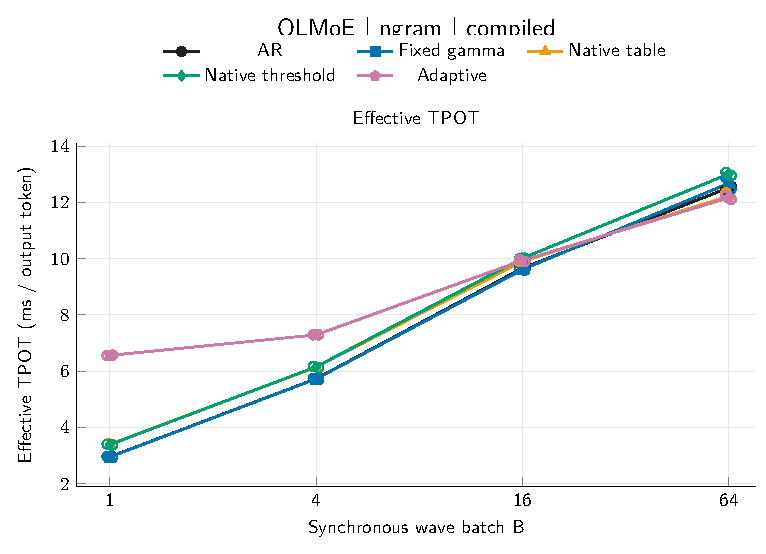
\includegraphics[width=0.64302\textwidth]{figures/F3_executed_policies.pdf}
\caption{F3: actual compiled five-policy evaluation on the same 64-request evaluation population at each $B$, with 128 forced output tokens/request. Open points retain both run values; lines are medians. Selected fixed $\gamma=0$ is executed separately from AR. Native tables and fixed-budget adaptive execution have different graph/production boundaries. Shared resident engines and continuous estimator state are not independent engine repeats; no confidence intervals or significance claim are inferred.}
\label{fig:f3}
\end{figure*}

\subsection{Frozen selection and executed population}
Development effective TPOT, weighted equally over $B=1,4,16,64$, selects static $\gamma=0$ and threshold cutoff zero (all off). The unrestricted table selects caps 0/4/7 for active batches 1--15/16--63/64. AR and static use separate $G=0$ engines; the all-off threshold retains its $G_{\rm eng}=7$ PIECEWISE table engine and is not equivalent to AR. The evaluation uses workload entries 64--127, disjoint from development entries 0--63, with development-prompt shape warmup. Historical general warmup exposed 48 evaluation prompts, so this is not a whole-pipeline prompt-unseen test. All five arms complete four batches and two repeats: 40 run records, zero exclusions, 64 requests and 8,192 emitted tokens/run. Repeats share resident engines; estimator state is continuous, and sequential run windows remain a limitation.

\subsection{TPOT improvement does not imply policy-level benefit}
The declared equal-batch mean of run-median effective TPOT is 7.7149/7.7405/7.9179/8.1410/8.9891\,ms for AR/static/unrestricted/threshold/adaptive, respectively (Figure~\ref{fig:f3}). Thus full-budget adaptation does not outperform selected static ordinary decoding on this objective. At $B=64$, adaptive/static TPOT is 0.9596, but population throughput is 0.9484 and energy/token is 1.0834 (Table~\ref{tab:policytradeoff}). This is a measured tradeoff in the present n-gram domain, not evidence that dynamic selection is generally ineffective.

\begin{table}[t]
\centering\small
\caption{Actual adaptive/static ratios of two-run medians. Lower TPOT and J/token are better; higher throughput is better. Population throughput includes inter-wave gaps; energy uses the validated device-counter span.}
\label{tab:policytradeoff}
\begin{tabular}{@{}rrrr@{}}
\toprule
$B$ & Effective TPOT & Population TPS & J/token \\\midrule
1 & 2.2276 & 0.4605 & 2.3932 \\
4 & 1.2737 & 0.7458 & 1.3504 \\
16 & 1.0337 & 0.9168 & 1.0553 \\
64 & 0.9596 & 0.9484 & 1.0834 \\
\bottomrule
\end{tabular}
\end{table}

\paragraph{F4: measured policy energy} All 40 device-counter spans are valid and include inter-wave gaps, with endpoints distinct from the runner population-wall clock. Adaptive uses more J/token than static at every tested batch. At $B=64$, its two raw values are 0.064076/0.064191 versus static 0.059959/0.058440\,J/token. These are whole-device, non-idle-subtracted observations, not whole-system energy; raw repeats and the separate wave-window metric are retained. They do not isolate graph, drafting, or CPU causes.

\paragraph{F6: control and discarded proposals} Adaptive decision-call means range from 39.70 to 52.14\,$\mu$s across the eight runs. Both $B=1$ runs always select cap seven. The discarded/available proposal fraction is zero there, 0.422666 in both $B=4$ runs, 0.731301/0.689627 at $B=16$, and 0.430243 in both $B=64$ runs. Counts cover scheduled decode steps including terminal/drain steps; CPU means cover actually timed calls. Missing native decision timing is not zero. Discarded tokens do not measure wasted GPU time or energy. Decision, wrapper, and schedule timers are nested; they cannot be summed or subtracted from wall time to infer an uninstrumented policy. Total observer perturbation still requires an ablation.

\subsection{Evidence scope and remaining validation}
F1 tests occupancy/component costs and diagnoses physical participation; F2 characterizes static compiled waves. F3 now measures all five policies, with F4 policy energy and F6 adaptive control costs, without supporting an aggregate adaptive advantage here. F5 includes eager availability/offline tracking and compiled native acceptance-state observation: 240,254 recovered host steps, with 7,168 terminal request-steps censored. Those native runs did not update availability state or log adaptive predictions; they do not establish learned availability or method benefit. Separately, actual adaptive logging matches 19,759 post-step alpha values and 170 wave-end states; 19,419 scored decision steps give run-level request-weighted progress MAE 0.0603--0.2313 tokens/request-step against realized observations, not latent probabilities. The future-prefix reference on fixed trajectories remains an external diagnostic, not an F3 oracle curve, online strategy, or theoretical bound.

A natural-stop check completes 12 cells (AR/static/adaptive, $B=1,8$, two repeats, 16 requests/cell, 256-token cap) with zero failed, unfinished, or missing requests: at $B=1$, each AR/static run has 4 EOS and 12 capped outputs versus adaptive 2/14; at $B=8$, every arm/run has 3/13. Fixed-first-eight inspection at $B=1$, repeat 0, chosen from workload offset 64 independently of outcomes, finds instruction violations and unsupported personal achievements across arms and capped incomplete code; these observations establish neither task correctness nor quality/distributional equivalence. All arms share device capacity and a declared 6\,GiB KV allocation, not equalized total residency. Combined weights, metadata, achieved KV, and startup/compile costs remain separately scoped. Broader neural sources, targets, code/summarization workloads, and continuous-load tests are still required; their availability and costs must be measured rather than assumed. The present negative adaptive comparison motivates these already planned tests without changing the declared objective or discarding unfavorable runs.

\section{Related Work}
MoESD explains batch-dependent expert activation and fits performance parameters~\cite{moesd}. Our reviewed evidence does not locate an online optimal-length controller; this does not rule out unpublished implementations.

Cascade implements utility-driven adaptive MoE speculation with test-and-set, disabling, back-off, and hill-climbing~\cite{cascade}. Table~\ref{tab:t2actions} contrasts its feedback with our batch state and calibrated costs. We neither reproduce it nor claim superiority; controller results are scoped to the four implemented AR/native baselines.

AdaEAGLE learns draft length~\cite{adaeagle}; SpecDec++ predicts acceptance and stops by accumulated rejection risk~\cite{specdecpp}; DISCO classifies draft continuation~\cite{disco}. Their information and training costs differ. EAGLE-3 generates drafts but does not establish our controller's value~\cite{eagle3}.

Native vLLM already supports batch-only adaptation~\cite{vllmdynamic,vllmconfig}. MoE-Spec changes verification expert budgets with a quality tradeoff~\cite{moespec}; we retain target routing and make no expert-dropping claim.

\section{Conclusion}
The measured OLMoE/n-gram setting separates configured cap, useful progress, expert participation, and service cost. Actual rows improve held-out-cap occupancy prediction; compiled padding expands physical participation. Distinct experts predict eager and graph layer intervals without identifying a broad compute transition or full-model fixed-cost dominance. Eager and compiled service give different throughput directions without isolating a graph-only cause; throughput, TPOT, and energy also differ. The executed five-policy comparison finds no aggregate adaptive advantage over selected static ordinary decoding; its large-batch TPOT gain trades against throughput and energy. The small natural-stop check retains task-quality limitations; broader neural/code/summarization tests remain necessary, with availability measured rather than assumed.

\bibliographystyle{IEEEtran}
\bibliography{refs}
\end{document}
